% Created by tikzDevice version 0.10.1 on 2017-11-10 10:35:56
% !TEX encoding = UTF-8 Unicode
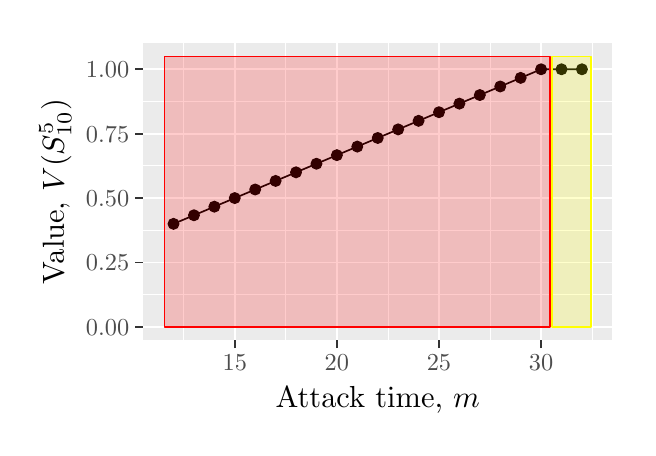
\begin{tikzpicture}[x=1pt,y=1pt]
\definecolor{fillColor}{RGB}{255,255,255}
\path[use as bounding box,fill=fillColor,fill opacity=0.00] (0,0) rectangle (216.81,144.54);
\begin{scope}
\path[clip] (  0.00,  0.00) rectangle (216.81,144.54);
\definecolor{drawColor}{RGB}{255,255,255}
\definecolor{fillColor}{RGB}{255,255,255}

\path[draw=drawColor,line width= 0.6pt,line join=round,line cap=round,fill=fillColor] (  0.00,  0.00) rectangle (216.81,144.54);
\end{scope}
\begin{scope}
\path[clip] ( 41.67, 31.53) rectangle (211.31,139.04);
\definecolor{fillColor}{gray}{0.92}

\path[fill=fillColor] ( 41.67, 31.53) rectangle (211.31,139.04);
\definecolor{drawColor}{RGB}{255,255,255}

\path[draw=drawColor,line width= 0.3pt,line join=round] ( 41.67, 48.05) --
	(211.31, 48.05);

\path[draw=drawColor,line width= 0.3pt,line join=round] ( 41.67, 71.32) --
	(211.31, 71.32);

\path[draw=drawColor,line width= 0.3pt,line join=round] ( 41.67, 94.59) --
	(211.31, 94.59);

\path[draw=drawColor,line width= 0.3pt,line join=round] ( 41.67,117.86) --
	(211.31,117.86);

\path[draw=drawColor,line width= 0.3pt,line join=round] ( 56.39, 31.53) --
	( 56.39,139.04);

\path[draw=drawColor,line width= 0.3pt,line join=round] ( 93.28, 31.53) --
	( 93.28,139.04);

\path[draw=drawColor,line width= 0.3pt,line join=round] (130.18, 31.53) --
	(130.18,139.04);

\path[draw=drawColor,line width= 0.3pt,line join=round] (167.07, 31.53) --
	(167.07,139.04);

\path[draw=drawColor,line width= 0.3pt,line join=round] (203.97, 31.53) --
	(203.97,139.04);

\path[draw=drawColor,line width= 0.6pt,line join=round] ( 41.67, 36.42) --
	(211.31, 36.42);

\path[draw=drawColor,line width= 0.6pt,line join=round] ( 41.67, 59.69) --
	(211.31, 59.69);

\path[draw=drawColor,line width= 0.6pt,line join=round] ( 41.67, 82.96) --
	(211.31, 82.96);

\path[draw=drawColor,line width= 0.6pt,line join=round] ( 41.67,106.23) --
	(211.31,106.23);

\path[draw=drawColor,line width= 0.6pt,line join=round] ( 41.67,129.50) --
	(211.31,129.50);

\path[draw=drawColor,line width= 0.6pt,line join=round] ( 74.83, 31.53) --
	( 74.83,139.04);

\path[draw=drawColor,line width= 0.6pt,line join=round] (111.73, 31.53) --
	(111.73,139.04);

\path[draw=drawColor,line width= 0.6pt,line join=round] (148.63, 31.53) --
	(148.63,139.04);

\path[draw=drawColor,line width= 0.6pt,line join=round] (185.52, 31.53) --
	(185.52,139.04);
\definecolor{drawColor}{RGB}{0,0,0}
\definecolor{fillColor}{RGB}{0,0,0}

\path[draw=drawColor,line width= 0.4pt,line join=round,line cap=round,fill=fillColor] (192.90,129.50) circle (  1.96);

\path[draw=drawColor,line width= 0.4pt,line join=round,line cap=round,fill=fillColor] (200.28,129.50) circle (  1.96);

\path[draw=drawColor,line width= 0.4pt,line join=round,line cap=round,fill=fillColor] ( 52.70, 73.65) circle (  1.96);

\path[draw=drawColor,line width= 0.4pt,line join=round,line cap=round,fill=fillColor] ( 60.08, 76.75) circle (  1.96);

\path[draw=drawColor,line width= 0.4pt,line join=round,line cap=round,fill=fillColor] ( 67.46, 79.86) circle (  1.96);

\path[draw=drawColor,line width= 0.4pt,line join=round,line cap=round,fill=fillColor] ( 74.83, 82.96) circle (  1.96);

\path[draw=drawColor,line width= 0.4pt,line join=round,line cap=round,fill=fillColor] ( 82.21, 86.06) circle (  1.96);

\path[draw=drawColor,line width= 0.4pt,line join=round,line cap=round,fill=fillColor] ( 89.59, 89.16) circle (  1.96);

\path[draw=drawColor,line width= 0.4pt,line join=round,line cap=round,fill=fillColor] ( 96.97, 92.27) circle (  1.96);

\path[draw=drawColor,line width= 0.4pt,line join=round,line cap=round,fill=fillColor] (104.35, 95.37) circle (  1.96);

\path[draw=drawColor,line width= 0.4pt,line join=round,line cap=round,fill=fillColor] (111.73, 98.47) circle (  1.96);

\path[draw=drawColor,line width= 0.4pt,line join=round,line cap=round,fill=fillColor] (119.11,101.57) circle (  1.96);

\path[draw=drawColor,line width= 0.4pt,line join=round,line cap=round,fill=fillColor] (126.49,104.68) circle (  1.96);

\path[draw=drawColor,line width= 0.4pt,line join=round,line cap=round,fill=fillColor] (133.87,107.78) circle (  1.96);

\path[draw=drawColor,line width= 0.4pt,line join=round,line cap=round,fill=fillColor] (141.25,110.88) circle (  1.96);

\path[draw=drawColor,line width= 0.4pt,line join=round,line cap=round,fill=fillColor] (148.63,113.99) circle (  1.96);

\path[draw=drawColor,line width= 0.4pt,line join=round,line cap=round,fill=fillColor] (156.00,117.09) circle (  1.96);

\path[draw=drawColor,line width= 0.4pt,line join=round,line cap=round,fill=fillColor] (163.38,120.19) circle (  1.96);

\path[draw=drawColor,line width= 0.4pt,line join=round,line cap=round,fill=fillColor] (170.76,123.29) circle (  1.96);

\path[draw=drawColor,line width= 0.4pt,line join=round,line cap=round,fill=fillColor] (178.14,126.40) circle (  1.96);

\path[draw=drawColor,line width= 0.4pt,line join=round,line cap=round,fill=fillColor] (185.52,129.50) circle (  1.96);

\path[draw=drawColor,line width= 0.6pt,line join=round] ( 52.70, 73.65) --
	( 60.08, 76.75) --
	( 67.46, 79.86) --
	( 74.83, 82.96) --
	( 82.21, 86.06) --
	( 89.59, 89.16) --
	( 96.97, 92.27) --
	(104.35, 95.37) --
	(111.73, 98.47) --
	(119.11,101.57) --
	(126.49,104.68) --
	(133.87,107.78) --
	(141.25,110.88) --
	(148.63,113.99) --
	(156.00,117.09) --
	(163.38,120.19) --
	(170.76,123.29) --
	(178.14,126.40) --
	(185.52,129.50) --
	(192.90,129.50) --
	(200.28,129.50);
\definecolor{drawColor}{RGB}{255,255,0}
\definecolor{fillColor}{RGB}{255,255,0}

\path[draw=drawColor,line width= 0.6pt,line join=round,fill=fillColor,fill opacity=0.20] (189.58, 36.42) rectangle (203.60,134.15);
\definecolor{drawColor}{RGB}{255,0,0}
\definecolor{fillColor}{RGB}{255,0,0}

\path[draw=drawColor,line width= 0.6pt,line join=round,fill=fillColor,fill opacity=0.20] ( 49.38, 36.42) rectangle (188.84,134.15);
\end{scope}
\begin{scope}
\path[clip] (  0.00,  0.00) rectangle (216.81,144.54);
\definecolor{drawColor}{gray}{0.30}

\node[text=drawColor,anchor=base east,inner sep=0pt, outer sep=0pt, scale=  0.88] at ( 36.72, 33.39) {0.00};

\node[text=drawColor,anchor=base east,inner sep=0pt, outer sep=0pt, scale=  0.88] at ( 36.72, 56.66) {0.25};

\node[text=drawColor,anchor=base east,inner sep=0pt, outer sep=0pt, scale=  0.88] at ( 36.72, 79.93) {0.50};

\node[text=drawColor,anchor=base east,inner sep=0pt, outer sep=0pt, scale=  0.88] at ( 36.72,103.20) {0.75};

\node[text=drawColor,anchor=base east,inner sep=0pt, outer sep=0pt, scale=  0.88] at ( 36.72,126.47) {1.00};
\end{scope}
\begin{scope}
\path[clip] (  0.00,  0.00) rectangle (216.81,144.54);
\definecolor{drawColor}{gray}{0.20}

\path[draw=drawColor,line width= 0.6pt,line join=round] ( 38.92, 36.42) --
	( 41.67, 36.42);

\path[draw=drawColor,line width= 0.6pt,line join=round] ( 38.92, 59.69) --
	( 41.67, 59.69);

\path[draw=drawColor,line width= 0.6pt,line join=round] ( 38.92, 82.96) --
	( 41.67, 82.96);

\path[draw=drawColor,line width= 0.6pt,line join=round] ( 38.92,106.23) --
	( 41.67,106.23);

\path[draw=drawColor,line width= 0.6pt,line join=round] ( 38.92,129.50) --
	( 41.67,129.50);
\end{scope}
\begin{scope}
\path[clip] (  0.00,  0.00) rectangle (216.81,144.54);
\definecolor{drawColor}{gray}{0.20}

\path[draw=drawColor,line width= 0.6pt,line join=round] ( 74.83, 28.78) --
	( 74.83, 31.53);

\path[draw=drawColor,line width= 0.6pt,line join=round] (111.73, 28.78) --
	(111.73, 31.53);

\path[draw=drawColor,line width= 0.6pt,line join=round] (148.63, 28.78) --
	(148.63, 31.53);

\path[draw=drawColor,line width= 0.6pt,line join=round] (185.52, 28.78) --
	(185.52, 31.53);
\end{scope}
\begin{scope}
\path[clip] (  0.00,  0.00) rectangle (216.81,144.54);
\definecolor{drawColor}{gray}{0.30}

\node[text=drawColor,anchor=base,inner sep=0pt, outer sep=0pt, scale=  0.88] at ( 74.83, 20.52) {15};

\node[text=drawColor,anchor=base,inner sep=0pt, outer sep=0pt, scale=  0.88] at (111.73, 20.52) {20};

\node[text=drawColor,anchor=base,inner sep=0pt, outer sep=0pt, scale=  0.88] at (148.63, 20.52) {25};

\node[text=drawColor,anchor=base,inner sep=0pt, outer sep=0pt, scale=  0.88] at (185.52, 20.52) {30};
\end{scope}
\begin{scope}
\path[clip] (  0.00,  0.00) rectangle (216.81,144.54);
\definecolor{drawColor}{RGB}{0,0,0}

\node[text=drawColor,anchor=base,inner sep=0pt, outer sep=0pt, scale=  1.10] at (126.49,  7.44) {Attack time, $m$};
\end{scope}
\begin{scope}
\path[clip] (  0.00,  0.00) rectangle (216.81,144.54);
\definecolor{drawColor}{RGB}{0,0,0}

\node[text=drawColor,rotate= 90.00,anchor=base,inner sep=0pt, outer sep=0pt, scale=  1.10] at ( 13.08, 85.29) {Value, $V(S_{ 10 }^{ 5 })$};
\end{scope}
\end{tikzpicture}
